\documentclass[12pt, a4paper]{article}

\usepackage{graphicx}
\usepackage[utf8]{inputenc}
\usepackage[italian]{babel}
\usepackage{hyperref}

%settings dei links
\hypersetup{
	colorlinks=true,
	linkcolor=black,
	urlcolor=red,
	pdftoolbar=true,
	pdfmenubar=true,
	pdftitle={English World},
	pdfauthor={Timoty Granziero, Elisa Giorio},
	pdfcreator={Timoty Granziero}	
}

\begin{document}

\frenchspacing
\begin{titlepage}
	\centering
	
\includegraphics[width=0.50\textwidth]{img/logo_unipd_color.png}\par\vspace{1cm} %logo
	
	{\LARGE\bfseries Progetto di Tecnologie Web \par}
	\vspace{1cm}
	{\Large\bfseries a.a. 2017/2018 \par}
	\vspace{2cm}
	
	{\Large Titolo della pagina web: \par}
	\vspace{0.5cm}
	
	{\LARGE\bfseries\itshape ENGLISH WORLD \par}
	
	\vfill 

	Autori: \par
	{\bfseries Elisa Giorio \par}
	{\bfseries Timoty Granziero \par}
	{\bfseries Edoardo Retis \par}
	
	\vfill

	Indirizzo del sito: \par
	\url{www.wikipedia.com}
	\vfill
	
	% Bottom of the page
	{\large \today\par}
	
\end{titlepage}

%indice
\tableofcontents 
\pagebreak

\begin{abstract}
Con questo progetto ci poniamo di illustrare le attività proposte da una scuola privata di lingua inglese. La nostra piattaforma dovrà dare tutte le informazioni che uno studente, di qualsiasi età, cercherà in un sito; allo stesso tempo dovrà dare strumenti facili ai docenti per inserire le informazioni sulle lezioni, aule usate e sugli esami.\par
Ci saranno pagine dedicate ai corsi, per capire qual è il nostro livello di inglese; altre destinate alle lezioni e successivamente agli esami.
\end{abstract}

\section{Introduzione}

\subsection{Utenti destinatari}
Il sito internet sviluppato non vuole raggiungere una sola categoria di utenti, ma è destinato a chiunque cerchi una scuola di inglese.  Inoltre ogni utente potrà facilmente raccogliere le informazioni che cerca, sia che sia al primo accesso, sia un utente abituale del sito.\par
Il sito internet si propone come obbiettivo il raggiungimento di un utenza non solo giovane, bensì di qualsiasi età avvicinandola così alla tematica trattata.

\subsection{Lo scopo del sito web}
Il sito si propone di stabilire un canale di comunicazione sicuro e semplice tra la scuola e gli studenti che lo frequentano. A tal proposito abbiamo progettato il sito web concentrandoci sugli aspetti che potessero non solo dare all’utente la risposta che cerca, ma anche fornire un modo chiaro per farlo. Il sito web di fatto è semplice ed intuitivo, con una grafica non invasiva ma non per questo da ritenersi obsoleta.\par
\bigskip
All’interno del sito l’utente proverà una serie di corsi accompagnati da una breve descrizione. Una volta scelto il corso, ci saranno pagine dedicate allo svolgimento dei corsi e successivamente dell’esame.\par
\bigskip
Oltre alla parte utente, il sito possiede anche una parte docente, dove proprio quest’ultimi possono prenotare aule per le lezioni o inserire gli orari e date degli esami.
Nei seguenti paragrafi verrà descritta la struttura del sito internet e suoi dettagli tecnici, elencando le tecnologie usate e le funzioni a disposizione. Verrà in particolar modo commentata l’accessibilità e l’usabilità del sito dimostrando quanto il progetto sia in linea con i moderni standard di progettazione.

\section{Gruppo di lavoro}
Al momento della conformazione del gruppo, ogni componente ha potuto decidere quale parte del progetto avrebbe preferito curare e realizzare. 
Il lavoro è stato così suddiviso:
\begin{itemize}
	\item Elisa Giorio:
	\item Timoty Granziero:
	\item Edoardo Retis:
\end{itemize}

Per quanto riguarda la condivisione del materiale è stata usata la piattaforma di GitHub.

\section{Gerarchia dei file}

\subsection{Rappresentazione grafica}

\subsection{Organizzazione interna}
 
\pagebreak %da vedere se ometterlo

\section{Progettazione concettuale}
Tutte le pagine principali seguono lo stesso schema ed è quello visto a lezione:
\begin{itemize}
	\item \textit{Header}: dove sono presenti logo e titolo della pagina web;
	\item \textit{Path}: indica dove ci troviamo all'interno del sito;
	\item \textit{Menù}: menù a pannelli che indica quali pagine sono accessibili;
	\item \textit{Corpo}: contiene i contenuti della pagina;
	\item \textit{Footer}: utilizzato per inserire i loghi della validazione forniti da w3c, e il file .js per l’ultima modifica della pagina
\end{itemize}

\begin{center}
	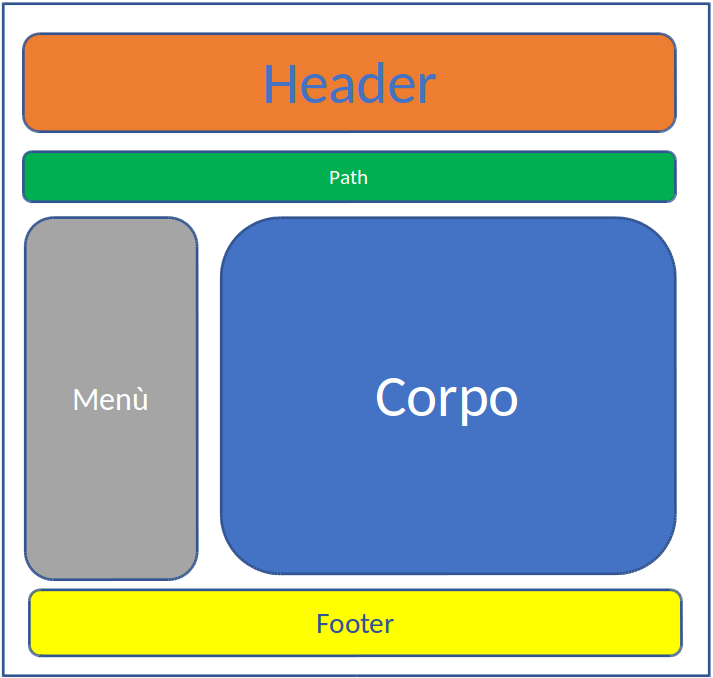
\includegraphics[height=9cm]{img/prog.png}
\end{center}

\section{Progettazione Logica}
\subsection{Parte utente}
\subsection{Parte Docente}
\subsection{Parte admin}

\section{Presentazione}

\section{Comportamento}
Si è scelto di utilizzare le tecnologie principali necessarie per lo sviluppo web, senza
scomodare framework o altre librerie che per l'uso praticamente nullo che ne avremmo fatto
sarebbe stato un inutile incremento dei tempi di risposta della pagina web.

\subsection{Uso di Javascript}
Javascript viene usato principalmente per due script: l'ultima modifica (nel file \textit{ultima\_modifica.js}), e come codice embedded nel file \textit{corsi.php}.
\begin{itemize}
	\item \textbf{ultima\_modifica.js}: in questo script viene aggiornata la data di ultima modifica del file dove è chiamata \texttt{lastModify()}.
	\item \textbf{corsi.php}: in questa pagina, viene utilizzato uno script che visualizza la posizione della sede immaginaria (esattamente quella della 
	Torre Archimede di Padova) attraverso un frame di \textit{Google Maps}.
\end{itemize}

\subsection{Uso di PHP}
La parte relativa a PHP è piuttosto consistente. Nella cartella \textit{presets}, sono presenti
alcuni script che, se inclusi tramite il comando \texttt{include()} di PHP, generano dimanicamente
una parte della pagina. \par
\smallskip
Nei file \textbf{header.php}, \textbf{footer.php} e \textbf{menu.php} generano rispettivamente la prima 
parte della pagina, il menu (assegnando dinamicamente valori di \texttt{tabindex} e la scheda attiva). \par
\smallskip
Nella cartella \textit{script}, sono presenti diversi script .php che eseguono controlli e comandi. Per interfacciarsi al database, si è scelto di utilizzare la libreria \texttt{mysqli}.\par
\smallskip
In \textbf{benvenuto.php} è un semplice script che genera codice relativo al login: chiede di accedere
in caso non ci sia un utente loggato, e da la possibilità di uscire in caso contrario. \textbf{logout.php} viene lanciato quando un utente loggato clicca su \texttt{Esci}. \par
Il file \textbf{validate\_form.php} serve a convalidare se il login avviene con successo o meno, e segnalare
gli eventuali errori. Infine, \mbox{\textbf{validate\_prenotation.php}} e \mbox{\textbf{validate\_prenotation\_exams.php}} validano le prenotazioni relative rispettivamente alle lezioni e agli esami (per 
evitare) sovrapposizioni), e in caso il controllo non riscontri problemi, le lezioni vengono inserite nel database.



\subsection{Uso di MySQL}
Come DBMS è stato scelto di utilizzare \texttt{MySQL}. Il database utilizzato è chiamato 
come il nome utente di laboratorio usato per la consegna: \textit{tgranzie}.\par 
I file utilizzati per popolare il database sono nella cartella \mbox{\textit{database}}:
\mbox{\textit{table.sql}} per le tabelle, e \mbox{\textit{input.sql}} per il popolamento. 
Ecco l'elenco delle tabelle utilizzate con una breve descrizione: \texttt{aule} contiene 
i dati relativi alle aule delle lezioni; \texttt{corsi} 
contiene l'elenco dei corsi disponibili nella scuola; in \texttt{docenti} ci sono i dati relativi 
ai docenti, comprese le credenziali per effettuare il login; in \texttt{esami} c'è la lista degli
esami relativi ai corsi; in \texttt{lezioni} le prenotazioni delle lezioni relative ai corsi.


\section{Validazione}

\section{Accessibilità}

\section{Usabilità}

\section{Considerazioni finali}

\end{document}